\documentclass[12pt]{article}
\usepackage{amsmath, amssymb, amsthm, geometry, tikz, enumitem, xcolor}
\geometry{letterpaper, margin=1in}

\title{Homework Chapter 1: Sets, Subsets, and Set Operations}
\author{Tashfeen Omran}
\date{September 2026}

\begin{document}
\maketitle
\tableofcontents
\newpage

\section{Part 1: Comprehensive Introduction, Context, and Prerequisites}

\subsection{Core Concepts}
The foundation of modern mathematical structure rests upon the concept of \textbf{sets}. A set is a well-defined collection of distinct objects, which are referred to as its \textbf{elements} or \textbf{members}. If an object $x$ is an element of a set $A$, we write $x \in A$. If it is not, we write $x \notin A$. Sets are typically denoted by uppercase letters (e.g., $A, B, C$), while elements are often denoted by lowercase letters (e.g., $a, b, c$). 

We typically describe sets using two primary methods:
\begin{enumerate}
    \item \textbf{The Roster Method:} Explicitly listing elements within curly braces, e.g., $A = \{1, 2, 3\}$.
    \item \textbf{Set-Builder Notation:} Defining a set by a property its elements must satisfy, e.g., $S = \{x \in \mathbb{R} : x > 0\}$, read as ``the set of all $x$ in the real numbers such that $x$ is greater than 0.''
\end{enumerate}

Key properties and related structures include:
\begin{itemize}
    \item \textbf{Cardinality:} The number of elements in a finite set $S$, denoted as $|S|$.
    \item \textbf{Subsets:} Set $A$ is a subset of $B$ (denoted $A \subseteq B$) if every element of $A$ is also in $B$. If $A \subseteq B$ but $A \neq B$, $A$ is a \textbf{proper subset} of $B$ (denoted $A \subset B$).
    \item \textbf{The Empty Set:} A unique set containing no elements, denoted as $\emptyset$ or $\{\}$.
    \item \textbf{Power Set:} The set of all subsets of a given set $A$, denoted $\mathcal{P}(A)$.
\end{itemize}

\subsection{Intuition and Derivation}
Set theory provides a universal language for mathematics, akin to how the alphabet provides a foundation for written language. The intuition behind set operations closely mirrors basic logical connectives:
\begin{itemize}
    \item \textbf{Union ($A \cup B$):} Elements in $A$ \textit{or} $B$ (logical OR).
    \item \textbf{Intersection ($A \cap B$):} Elements in \textit{both} $A$ \textit{and} $B$ (logical AND).
    \item \textbf{Difference ($A - B$):} Elements in $A$ \textit{but not} in $B$.
    \item \textbf{Complement ($\overline{A}$):} Elements in the Universal set $U$ that are \textit{not} in $A$ (logical NOT).
\end{itemize}
The cardinality of a power set is derived intuitively through combinatorics: for a set of $n$ elements, forming a subset requires making a binary ``yes/no'' choice for each element. Thus, there are $2 \times 2 \times \dots \times 2 = 2^n$ possible subsets, giving the formula $|\mathcal{P}(A)| = 2^{|A|}$.

\subsection{Historical Context and Motivation}
Set theory was formalized in the late 19th century, primarily by the German mathematician Georg Cantor. Before Cantor, mathematicians studied specific collections (like real numbers or functions) but lacked a rigorous framework to discuss infinite collections mathematically. Cantor's work on trigonometric series led him to formally define sets and prove that infinite sets can have different sizes (e.g., there are ``more'' real numbers than integers). While Cantor's ``naive'' set theory initially suffered from logical paradoxes (such as Russell's Paradox), it motivated the axiomatic set theories (like Zermelo-Fraenkel) that now form the absolute bedrock of modern mathematics.

\subsection{Key Formulas and Standard Sets}
\begin{itemize}
    \item $\mathbb{N}$: Natural numbers (positive integers) $\{1, 2, 3, \dots\}$.
    \item $\mathbb{Z}$: Integers $\{\dots, -2, -1, 0, 1, 2, \dots\}$.
    \item $\mathbb{Q}$: Rational numbers $\{ \frac{m}{n} : m, n \in \mathbb{Z}, n \neq 0 \}$.
    \item $\mathbb{R}$: Real numbers (all rational and irrational numbers).
    \item $\mathbb{C}$: Complex numbers $\{a + bi : a, b \in \mathbb{R}, i = \sqrt{-1}\}$.
    \item \textbf{Power Set Cardinality:} $|\mathcal{P}(A)| = 2^{|A|}$.
\end{itemize}

\subsection{Prerequisites}
To master these sections, one must possess:
\begin{enumerate}
    \item \textbf{Basic Algebra:} Ability to solve linear, quadratic, and absolute value equations (e.g., $x^2 - x = 0$ or $|x| = 2$).
    \item \textbf{Inequalities:} Understanding of strict and non-strict inequalities (e.g., $-4 < n \le 4$).
    \item \textbf{Number Systems:} Familiarity with integers, rational numbers, and real numbers to accurately identify domain restrictions in set-builder notation.
\end{enumerate}

\newpage
\section{Part 2: Detailed Homework Solutions}

\subsection{Section 1.1 Exercises (Describing a Set)}

\textbf{1.1. Which of the following are sets?} \\
(a) $1, 2, 3$ \quad (b) $\{1, 2\}, 3$ \quad (c) $\{\{1\}, 2\}, 3$ \quad (d) $\{1, \{2\}, 3\}$ \quad (e) $\{1, 2, a, b\}$ \\
\textbf{Solution:} By standard mathematical convention, a set is denoted by enclosing its elements in curly braces $\{\}$. 
Choices (a), (b), and (c) are simply comma-separated lists ending with a number outside of any bounding braces, so they do not represent a single set. 
Choices (d) and (e) are collections properly bounded by braces.
\textbf{Final Answer:} (d) and (e).

\vspace{0.5cm}
\textbf{1.2. Let $S = \{-2, -1, 0, 1, 2, 3\}$. Describe each of the following sets as $\{x \in S : p(x)\}$, where $p(x)$ is some condition on $x$.} \\
(a) $A = \{1, 2, 3\}$ \quad (b) $B = \{0, 1, 2, 3\}$ \quad (c) $C = \{-2, -1\}$ \quad (d) $D = \{-2, 2, 3\}$ \\
\textbf{Solution:}
\begin{itemize}
    \item[(a)] $A$ contains only the positive integers in $S$. \textbf{Answer:} $A = \{x \in S : x > 0\}$
    \item[(b)] $B$ contains the non-negative integers in $S$. \textbf{Answer:} $B = \{x \in S : x \ge 0\}$
    \item[(c)] $C$ contains the strictly negative integers in $S$. \textbf{Answer:} $C = \{x \in S : x < 0\}$
    \item[(d)] $D$ contains elements whose absolute value is $2$, along with $3$. \textbf{Answer:} $D = \{x \in S : |x| = 2 \text{ or } x = 3\}$
\end{itemize}

\vspace{0.5cm}
\textbf{1.3. Determine the cardinality of each of the following sets:} \\
(a) $A = \{1, 2, 3, 4, 5\}$ \quad (b) $B = \{0, 2, 4, \dots, 20\}$ \quad (c) $C = \{25, 26, 27, \dots, 75\}$ \\
(d) $D = \{\{1, 2\}, \{1, 2, 3, 4\}\}$ \quad (e) $E = \{\emptyset\}$ \quad (f) $F = \{2, \{2, 3, 4\}\}$ \\
\textbf{Solution:}
\begin{itemize}
    \item[(a)] Counting elements directly gives $5$. \textbf{Answer:} $|A| = 5$
    \item[(b)] The set is the even numbers from $0$ to $20$. Formula: $\frac{20-0}{2} + 1 = 11$. \textbf{Answer:} $|B| = 11$
    \item[(c)] Consecutive integers from $25$ to $75$. Formula: $75 - 25 + 1 = 51$. \textbf{Answer:} $|C| = 51$
    \item[(d)] The set contains exactly two elements, both of which happen to be sets. \textbf{Answer:} $|D| = 2$
    \item[(e)] The set contains one element (the empty set). \textbf{Answer:} $|E| = 1$
    \item[(f)] The set contains the integer $2$ and the set $\{2, 3, 4\}$. \textbf{Answer:} $|F| = 2$
\end{itemize}

\vspace{0.5cm}
\textbf{1.4. Write each of the following sets by listing its elements within braces.} \\
\textbf{Solution:}
\begin{itemize}
    \item[(a)] $A = \{n \in \mathbb{Z} : -4 < n \le 4\}$. The integers strictly greater than $-4$ and up to $4$. \\
    \textbf{Answer:} $A = \{-3, -2, -1, 0, 1, 2, 3, 4\}$
    \item[(b)] $B = \{n \in \mathbb{Z} : n^2 < 5\}$. The squares less than $5$ are $0, 1, 4$. This corresponds to roots $-2, -1, 0, 1, 2$. \\
    \textbf{Answer:} $B = \{-2, -1, 0, 1, 2\}$
    \item[(c)] $C = \{n \in \mathbb{N} : n^3 < 100\}$. The natural numbers (starting from $1$) whose cubes are less than $100$. $1^3=1, 2^3=8, 3^3=27, 4^3=64, 5^3=125$. \\
    \textbf{Answer:} $C = \{1, 2, 3, 4\}$
    \item[(d)] $D = \{x \in \mathbb{R} : x^2 - x = 0\}$. Factoring gives $x(x - 1) = 0$, so $x = 0$ or $x = 1$. Both are real. \\
    \textbf{Answer:} $D = \{0, 1\}$
    \item[(e)] $E = \{x \in \mathbb{R} : x^2 + 1 = 0\}$. Solving gives $x^2 = -1 \implies x = \pm i$. There are no \textit{real} solutions. \\
    \textbf{Answer:} $E = \emptyset$
\end{itemize}

\vspace{0.5cm}
\textbf{1.5. Write each of the following sets in the form $\{x \in \mathbb{Z} : p(x)\}$.} \\
\textbf{Solution:}
\begin{itemize}
    \item[(a)] $A = \{-1, -2, -3, \dots\}$. These are all strictly negative integers. \\
    \textbf{Answer:} $A = \{x \in \mathbb{Z} : x \le -1\}$
    \item[(b)] $B = \{-3, -2, \dots, 3\}$. These are all integers between $-3$ and $3$ inclusive. \\
    \textbf{Answer:} $B = \{x \in \mathbb{Z} : -3 \le x \le 3\}$ (or $\{x \in \mathbb{Z} : |x| \le 3\}$)
    \item[(c)] $C = \{-2, -1, 1, 2\}$. These are integers whose absolute values are $1$ or $2$. \\
    \textbf{Answer:} $C = \{x \in \mathbb{Z} : 1 \le |x| \le 2\}$
\end{itemize}

\vspace{0.5cm}
\textbf{1.6. The set $E = \{2x : x \in \mathbb{Z}\}$ can be described by listing its elements, namely $E = \{\dots, -4, -2, 0, 2, 4, \dots\}$. List the elements of the following sets in a similar manner.} \\
\textbf{Solution:}
\begin{itemize}
    \item[(a)] $A = \{2x + 1 : x \in \mathbb{Z}\}$. These are the odd integers. \\
    \textbf{Answer:} $A = \{\dots, -3, -1, 1, 3, 5, \dots\}$
    \item[(b)] $B = \{4n : n \in \mathbb{Z}\}$. These are multiples of $4$. \\
    \textbf{Answer:} $B = \{\dots, -8, -4, 0, 4, 8, \dots\}$
    \item[(c)] $C = \{3q + 1 : q \in \mathbb{Z}\}$. These are integers congruent to $1$ modulo $3$. \\
    \textbf{Answer:} $C = \{\dots, -5, -2, 1, 4, 7, \dots\}$
\end{itemize}

\vspace{0.5cm}
\textbf{1.7. Describe the following sets in a similar manner by defining a condition.} \\
\textbf{Solution:}
\begin{itemize}
    \item[(a)] $A = \{\dots, -4, -1, 2, 5, 8, \dots\}$. The difference between consecutive elements is $3$. At $x=0$, let $y=2$. The mapping is $y = 3x + 2$. \\
    \textbf{Answer:} $A = \{3x + 2 : x \in \mathbb{Z}\}$
    \item[(b)] $B = \{\dots, -10, -5, 0, 5, 10, \dots\}$. These are multiples of $5$. \\
    \textbf{Answer:} $B = \{5x : x \in \mathbb{Z}\}$
    \item[(c)] $C = \{1, 8, 27, 64, 125, \dots\}$. These are perfect cubes of positive integers. \\
    \textbf{Answer:} $C = \{x^3 : x \in \mathbb{N}\}$
\end{itemize}

\vspace{0.5cm}
\textbf{1.8. Let $A = \{n \in \mathbb{Z} : 2 \le |n| < 4\}$, $B = \{x \in \mathbb{Q} : 2 < x \le 4\}$, \\ 
$C = \{x \in \mathbb{R} : x^2 - (2 + \sqrt{2})x + 2\sqrt{2} = 0\}$, and $D = \{x \in \mathbb{Q} : x^2 - (2 + \sqrt{2})x + 2\sqrt{2} = 0\}$.} \\
\textbf{Solution:}
First, let's explicitly find the sets $A, C$, and $D$.
For $A$: The integers whose absolute value is $\ge 2$ and $< 4$ are $\pm 2, \pm 3$. Thus $A = \{-3, -2, 2, 3\}$.
For $C, D$: Solve the quadratic using factoring. The equation is $x^2 - 2x - x\sqrt{2} + 2\sqrt{2} = 0 \implies x(x - 2) - \sqrt{2}(x - 2) = 0 \implies (x - \sqrt{2})(x - 2) = 0$. Roots are $2$ and $\sqrt{2}$. Since $C$ takes real numbers, $C = \{2, \sqrt{2}\}$. Since $D$ takes only rational numbers and $\sqrt{2}$ is irrational, $D = \{2\}$.
\begin{itemize}
    \item[(a)] Describe $A$ by listing elements. \textbf{Answer:} $A = \{-3, -2, 2, 3\}$
    \item[(b)] Give three elements in $B$ but not in $A$. \textbf{Answer:} $2.5, 3, 3.5$ (Note: 3 is in A, so $3$ is incorrect. Correct examples: $2.5, 3.5, 4$). Let's use $\frac{5}{2}, \frac{7}{2}, 4$.
    \item[(c)] Describe $C$ by listing elements. \textbf{Answer:} $C = \{2, \sqrt{2}\}$
    \item[(d)] Describe $D$ in another manner. \textbf{Answer:} $D = \{2\}$
    \item[(e)] Determine cardinality of $A, C, D$. \textbf{Answer:} $|A| = 4, |C| = 2, |D| = 1$
\end{itemize}

\vspace{0.5cm}
\textbf{1.9. For $A = \{2, 3, 5, 7, 8, 10, 13\}$, let \\
$B = \{x \in A : x = y + z \text{ where } y, z \in A\}$, and $C = \{r \in B : r + s \in B \text{ for some } s \in B\}$. Determine $C$.} \\
\textbf{Solution:}
First, find $B$. We look for elements in $A$ that can be formed by adding any two elements of $A$ (including adding an element to itself).
\begin{itemize}
    \item $2+3=5 \implies 5 \in B$
    \item $2+5=7 \implies 7 \in B$
    \item $3+5=8 \implies 8 \in B$
    \item $5+5=10 \implies 10 \in B$ (and $3+7=10$, $2+8=10$)
    \item $5+8=13 \implies 13 \in B$ (and $3+10=13$)
\end{itemize}
Thus, $B = \{5, 7, 8, 10, 13\}$.
Next, find $C$. We take elements $r \in B$ such that $r+s$ is also in $B$ for some $s \in B$.
\begin{itemize}
    \item Let $r = 5$. If $s = 5 \in B$, $r+s = 10 \in B$. Thus, $5 \in C$.
    \item Let $r = 7$. Smallest $s \in B$ is $5$. $7+5=12 \notin B$. $7+7=14 \notin B$. Thus, $7 \notin C$.
    \item Let $r = 8$. If $s = 5 \in B$, $8+5 = 13 \in B$. Thus, $8 \in C$.
    \item Let $r = 10$. Smallest sum is $10+5=15 \notin B$. Thus, $10 \notin C$.
    \item Let $r = 13$. Smallest sum is $13+5=18 \notin B$. Thus, $13 \notin C$.
\end{itemize}
\textbf{Final Answer:} $C = \{5, 8\}$

\subsection{Section 1.2 Exercises (Subsets)}

\textbf{1.10. Give examples of three sets $A, B$, and $C$ such that:} \\
\textbf{Solution:}
\begin{itemize}
    \item[(a)] $A \subseteq B \subset C$. \\
    \textbf{Answer:} $A = \{1\}, B = \{1, 2\}, C = \{1, 2, 3\}$.
    \item[(b)] $A \in B, B \in C$ and $A \notin C$. \\
    \textbf{Answer:} $A = \{1\}, B = \{\{1\}\}, C = \{\{\{1\}\}\}$. (Note that $A \notin C$ because the only element in $C$ is $B = \{\{1\}\}$, not $A = \{1\}$).
    \item[(c)] $A \in B$ and $A \subset C$. \\
    \textbf{Answer:} $A = \{1\}, B = \{\{1\}\}, C = \{1, 2\}$. Here $A \in B$ as an element, and $A$ is a proper subset of $C$.
\end{itemize}

\vspace{0.5cm}
\textbf{1.11. Let $(a,b)$ be an open interval of real numbers and let $c \in (a,b)$. Describe an open interval $I$ centered at $c$ such that $I \subseteq (a,b)$.} \\
\textbf{Solution:}
Since $c$ is strictly between $a$ and $b$, the distances to the endpoints are $c-a > 0$ and $b-c > 0$. We want the radius of our new interval to not exceed the smaller of these two distances.
Let $\epsilon = \min(c-a, b-c)$.
\textbf{Answer:} $I = (c - \epsilon, c + \epsilon)$

\vspace{0.5cm}
\textbf{1.12. Which of the following sets are equal?} \\
$A = \{n \in \mathbb{Z} : |n| < 2\}$, $B = \{n \in \mathbb{Z} : n^3 = n\}$, $C = \{n \in \mathbb{Z} : n^2 \le n\}$, $D = \{n \in \mathbb{Z} : n^2 \le 1\}$, $E = \{-1, 0, 1\}$. \\
\textbf{Solution:}
Evaluate each set:
\begin{itemize}
    \item $A = \{-1, 0, 1\}$
    \item For $B$, solve $n^3 - n = 0 \implies n(n-1)(n+1) = 0 \implies n \in \{-1, 0, 1\}$. So $B = \{-1, 0, 1\}$.
    \item For $C$, solve $n^2 - n \le 0 \implies n(n-1) \le 0 \implies 0 \le n \le 1$. In integers, $C = \{0, 1\}$.
    \item For $D$, solve $n^2 \le 1 \implies -1 \le n \le 1 \implies D = \{-1, 0, 1\}$.
    \item $E = \{-1, 0, 1\}$.
\end{itemize}
\textbf{Answer:} Sets $A, B, D$, and $E$ are equal.

\vspace{0.5cm}
\textbf{1.13. For a universal set $U = \{1, 2, \dots, 8\}$ and two sets $A = \{1, 3, 4, 7\}$ and $B = \{4, 5, 8\}$, draw a Venn diagram.} \\
\textbf{Solution:}
First, we identify the intersections and relative complements:
$A \cap B = \{4\}$.
Elements only in $A$: $\{1, 3, 7\}$.
Elements only in $B$: $\{5, 8\}$.
Elements outside both ($U - (A \cup B)$): $\{2, 6\}$.
\begin{center}
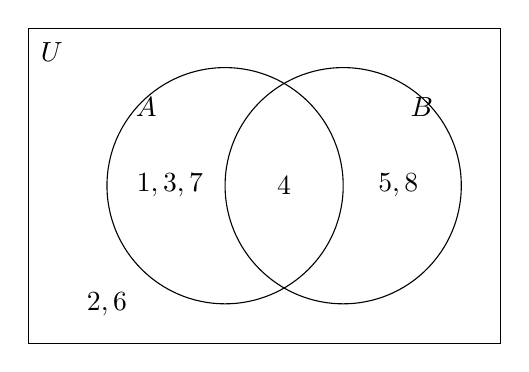
\begin{tikzpicture}
    % Draw Universal Set
    \draw (0,0) rectangle (6,4);
    \node at (0.3, 3.7) {$U$};
    
    % Draw Set A
    \draw (2.5,2) circle (1.5cm);
    \node at (1.5, 3) {$A$};
    
    % Draw Set B
    \draw (4,2) circle (1.5cm);
    \node at (5, 3) {$B$};
    
    % Place elements
    \node at (1.8, 2) {$1, 3, 7$};
    \node at (3.25, 2) {$4$};
    \node at (4.7, 2) {$5, 8$};
    
    % Place elements in U but outside A and B
    \node at (1, 0.5) {$2, 6$};
\end{tikzpicture}
\end{center}

\vspace{0.5cm}
\textbf{1.14. Find $\mathcal{P}(A)$ and $|\mathcal{P}(A)|$ for (a) $A = \{1, 2\}$ and (b) $A = \{\emptyset, 1, \{a\}\}$.} \\
\textbf{Solution:}
\begin{itemize}
    \item[(a)] $\mathcal{P}(A) = \{\emptyset, \{1\}, \{2\}, \{1, 2\}\}$. Cardinality is $2^2 = 4$.
    \item[(b)] $\mathcal{P}(A) = \{\emptyset, \{\emptyset\}, \{1\}, \{\{a\}\}, \{\emptyset, 1\}, \{\emptyset, \{a\}\}, \{1, \{a\}\}, \{\emptyset, 1, \{a\}\}\}$. Cardinality is $2^3 = 8$.
\end{itemize}

\vspace{0.5cm}
\textbf{1.15. Find $\mathcal{P}(A)$ for $A = \{0, \{0\}\}$.} \\
\textbf{Solution:} The elements are $0$ and $\{0\}$. \\
\textbf{Answer:} $\mathcal{P}(A) = \{\emptyset, \{0\}, \{\{0\}\}, \{0, \{0\}\}\}$

\vspace{0.5cm}
\textbf{1.16. Find $\mathcal{P}(\mathcal{P}(\{1\}))$ and its cardinality.} \\
\textbf{Solution:} First, $\mathcal{P}(\{1\}) = \{\emptyset, \{1\}\}$. This set has $2$ elements.
The power set of this set will have $2^2 = 4$ elements.
\textbf{Answer:} $\mathcal{P}(\mathcal{P}(\{1\})) = \{\emptyset, \{\emptyset\}, \{\{1\}\}, \{\emptyset, \{1\}\}\}$. Cardinality is $4$.

\vspace{0.5cm}
\textbf{1.17. Find $\mathcal{P}(A)$ and $|\mathcal{P}(A)|$ for $A = \{0, \emptyset, \{\emptyset\}\}$.} \\
\textbf{Solution:} $A$ has $3$ elements. $|\mathcal{P}(A)| = 2^3 = 8$. \\
\textbf{Answer:} $\mathcal{P}(A) = \{\emptyset, \{0\}, \{\emptyset\}, \{\{\emptyset\}\}, \{0, \emptyset\}, \{0, \{\emptyset\}\}, \{\emptyset, \{\emptyset\}\}, \{0, \emptyset, \{\emptyset\}\}\}$.

\vspace{0.5cm}
\textbf{1.18. For $A = \{x : x = 0 \text{ or } x \in \mathcal{P}(\{0\})\}$, determine $\mathcal{P}(A)$.} \\
\textbf{Solution:} Evaluate $\mathcal{P}(\{0\}) = \{\emptyset, \{0\}\}$.
So $A$ consists of $0$ combined with the elements of $\mathcal{P}(\{0\})$. Thus, $A = \{0, \emptyset, \{0\}\}$. Note that $0$ is an integer and $\{0\}$ is a set; they are distinct. Thus $|A| = 3$. \\
\textbf{Answer:} $\mathcal{P}(A) = \{\emptyset, \{0\}, \{\emptyset\}, \{\{0\}\}, \{0, \emptyset\}, \{0, \{0\}\}, \{\emptyset, \{0\}\}, \{0, \emptyset, \{0\}\}\}$.

\vspace{0.5cm}
\textbf{1.19. Give an example of a set $S$ such that:} \\
\textbf{Solution:}
\begin{itemize}
    \item[(a)] $S \subseteq \mathcal{P}(\mathbb{N})$: $S$ is a subset of the power set, meaning its elements must be subsets of $\mathbb{N}$. \textbf{Answer:} $S = \{\{1\}, \{2\}\}$
    \item[(b)] $S \in \mathcal{P}(\mathbb{N})$: $S$ is an element of the power set, meaning $S$ itself is a subset of $\mathbb{N}$. \textbf{Answer:} $S = \{1, 2\}$
    \item[(c)] $S \subseteq \mathcal{P}(\mathbb{N})$ and $|S|=5$. \textbf{Answer:} $S = \{\{1\}, \{2\}, \{3\}, \{4\}, \{5\}\}$
    \item[(d)] $S \in \mathcal{P}(\mathbb{N})$ and $|S|=5$. \textbf{Answer:} $S = \{1, 2, 3, 4, 5\}$
\end{itemize}

\vspace{0.5cm}
\textbf{1.20. Determine whether the following statements are true or false.} \\
\textbf{Solution:}
\begin{itemize}
    \item[(a)] \textit{If $\{1\} \in \mathcal{P}(A)$, then $1 \in A$ but $\{1\} \notin A$.} \\
    \textbf{False.} $\{1\} \in \mathcal{P}(A)$ implies $\{1\} \subseteq A$, which forces $1 \in A$. However, it is entirely possible that $\{1\} \in A$ as well (e.g., if $A = \{1, \{1\}\}$). The claim that it \textit{cannot} be in $A$ is false.
    \item[(b)] \textit{If $A, B, C$ are sets such that $A \subset \mathcal{P}(B) \subset C$ and $|A|=2$, then $|C|$ can be 5 but cannot be 4.} \\
    \textbf{True.} The symbol $\subset$ implies a \textit{proper} subset. Since $|A|=2$ and $A \subset \mathcal{P}(B)$, the cardinality of $\mathcal{P}(B)$ must be strictly greater than $2$. Since $|\mathcal{P}(B)|$ must be a power of $2$, the smallest it can be is $4$ (when $|B|=2$). If $|\mathcal{P}(B)| = 4$, and $\mathcal{P}(B) \subset C$ (proper), then $|C|$ must be strictly greater than $4$. Hence, $|C|$ cannot be 4, but it can be 5 (if we just add one element to form $C$).
    \item[(c)] \textit{If a set $B$ has one more element than a set $A$, then $\mathcal{P}(B)$ has at least two more elements than $\mathcal{P}(A)$.} \\
    \textbf{False.} Let $|A| = 0$ (so $A = \emptyset$). Then $|B| = 1$. $|\mathcal{P}(A)| = 2^0 = 1$ and $|\mathcal{P}(B)| = 2^1 = 2$. The difference is exactly $1$ element, not at least $2$.
    \item[(d)] \textit{If four sets $A, B, C, D$ are subsets of $\{1, 2, 3\}$ such that $|A|=|B|=|C|=|D|=2$, then at least two are equal.} \\
    \textbf{True.} The total number of subsets of size $2$ from a set of size $3$ is given by $\binom{3}{2} = 3$. Since there are only $3$ unique subsets of size $2$, choosing $4$ such subsets guarantees (by the Pigeonhole Principle) that at least two must be identical.
\end{itemize}

\vspace{0.5cm}
\textbf{1.21. Three subsets $A, B$ and $C$ of $\{1, 2, 3, 4, 5\}$ have the same cardinality. Furthermore: \\
(a) 1 belongs to $A$ and $B$ but not to $C$.\\
(b) 2 belongs to $A$ and $C$ but not to $B$.\\
(c) 3 belongs to $A$ and exactly one of $B$ and $C$.\\
(d) 4 belongs to an even number of $A, B, C$.\\
(e) 5 belongs to an odd number of $A, B, C$.\\
(f) The sums of the elements in two of the sets $A, B, C$ differ by 1. \\
What is $B$?} \\
\textbf{Solution:}
Let's deduce the sets.
From (a) and (b), we know $A$ contains $1, 2$. $B$ contains $1$ and not $2$. $C$ contains $2$ and not $1$.
From (c), $3 \in A$, and $3$ is in either $B$ or $C$ exclusively.
Assume $3 \in C$ (and not $B$). Then $A = \{1, 2, 3\}$. To have equal cardinality, all must have size $3$ (size cannot be $2$ since $A$ already has $3$ elements, and size $4$ forces contradictions with exclusivity).
If cardinality is $3$, $A$ is complete: $A = \{1, 2, 3\}$.
This means $4$ and $5$ are \textbf{not} in $A$.
From (d), $4$ is in an even number of sets. Since $4 \notin A$, $4$ must be in exactly $2$ sets: $B$ and $C$.
So far, $B = \{1, 4\}$ and $C = \{2, 3, 4\}$.
Since $C$ now has $3$ elements, it is complete.
From (e), $5$ is in an odd number of sets. It cannot be in $A$ or $C$, so it must be in exactly $1$ set: $B$.
Thus, $B = \{1, 4, 5\}$.
Let's verify (f) with the sums:
Sum of $A$ = $1+2+3 = 6$.
Sum of $B$ = $1+4+5 = 10$.
Sum of $C$ = $2+3+4 = 9$.
The sums of $B$ ($10$) and $C$ ($9$) differ by exactly $1$.
All conditions are perfectly satisfied.
\textbf{Final Answer:} $B = \{1, 4, 5\}$.

\subsection{Section 1.3 Exercises (Set Operations)}

\textbf{1.22. Let $U = \{1, 3, \dots, 15\}$ be the universal set, $A = \{1, 5, 9, 13\}$ and $B = \{3, 9, 15\}$. Determine the following:} \\
\textbf{Solution:} 
The universal set is the odd numbers up to $15$: $U = \{1, 3, 5, 7, 9, 11, 13, 15\}$.
\begin{itemize}
    \item[(a)] $A \cup B$: Elements in $A$ or $B$. \textbf{Answer:} $\{1, 3, 5, 9, 13, 15\}$
    \item[(b)] $A \cap B$: Elements in both. \textbf{Answer:} $\{9\}$
    \item[(c)] $A - B$: Elements in $A$ not in $B$. \textbf{Answer:} $\{1, 5, 13\}$
    \item[(d)] $B - A$: Elements in $B$ not in $A$. \textbf{Answer:} $\{3, 15\}$
    \item[(e)] $\overline{A}$: Elements in $U$ not in $A$. \textbf{Answer:} $\{3, 7, 11, 15\}$
    \item[(f)] $A \cap \overline{B}$: Elements in $A$ and not in $B$, which is identical to $A - B$. \textbf{Answer:} $\{1, 5, 13\}$
\end{itemize}

\vspace{0.5cm}
\textbf{1.23. Give examples of two sets $A$ and $B$ such that $|A - B| = |A \cap B| = |B - A| = 3$. Draw the accompanying Venn diagram.} \\
\textbf{Solution:}
We need $3$ elements strictly in $A$, $3$ strictly in $B$, and $3$ shared.
\textbf{Answer:} Let $A = \{1, 2, 3, 4, 5, 6\}$ and $B = \{4, 5, 6, 7, 8, 9\}$. 
\begin{center}
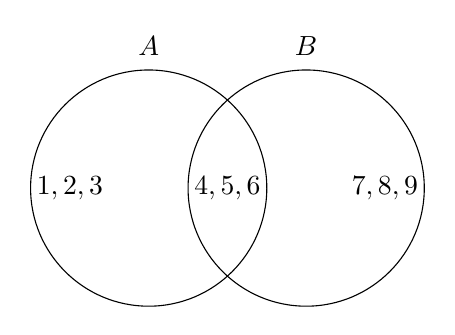
\begin{tikzpicture}
    \draw (1.5,0) circle (1.5cm);
    \draw (3.5,0) circle (1.5cm);
    \node at (0.5, 0) {$1, 2, 3$};
    \node at (2.5, 0) {$4, 5, 6$};
    \node at (4.5, 0) {$7, 8, 9$};
    \node at (1.5, 1.8) {$A$};
    \node at (3.5, 1.8) {$B$};
\end{tikzpicture}
\end{center}

\vspace{0.5cm}
\textbf{1.24. Give examples of three sets $A, B$, and $C$ such that $B \neq C$ but $B - A = C - A$.} \\
\textbf{Solution:}
We need $B$ and $C$ to differ, but their differences must lie entirely within $A$ so that when $A$ is subtracted, the remainders are identical.
\textbf{Answer:} Let $A = \{1, 2\}$, $B = \{1, 3\}$, and $C = \{2, 3\}$.
Here, $B \neq C$, but $B - A = \{3\}$ and $C - A = \{3\}$.

\vspace{0.5cm}
\textbf{1.25. Give examples of three sets $A, B$, and $C$ such that:} \\
\textbf{Solution:}
\begin{itemize}
    \item[(a)] $A \in B, A \subseteq C, B \not\subseteq C$. \\
    \textbf{Answer:} $A = \{1\}, B = \{\{1\}, 2\}, C = \{1\}$. 
    \item[(b)] $B \in A, B \subseteq C, A \cap C \neq \emptyset$. \\
    \textbf{Answer:} $B = \{1\}, A = \{\{1\}, 2\}, C = \{1, 2\}$. 
    \item[(c)] $A \in B, B \subseteq C, A \not\subseteq C$. \\
    \textbf{Answer:} $A = \{1\}, B = \{\{1\}\}, C = \{\{1\}\}$. (Here $1 \in A$, but $1 \notin C$, so $A \not\subseteq C$).
\end{itemize}

\vspace{0.5cm}
\textbf{1.26 - 1.28.} (Venn Diagram Construction Exercises) \\
\textbf{Solution Summary:} These exercises require drawing logical overlaps to confirm identities like De Morgan's Laws ($\overline{A \cup B} = \overline{A} \cap \overline{B}$). For example, in 1.27, providing $|A \cap B| = |A - B| = |B - A| = |\overline{A \cup B}| = 2$ means placing exactly $2$ elements in every atomic region of a two-set Venn diagram, yielding $8$ elements total in $U$.

\vspace{0.5cm}
\textbf{1.29. Let $A = \{\emptyset, \{\emptyset\}, \{\{\emptyset\}\}\}$.} \\
\textbf{Solution:}
\begin{itemize}
    \item[(a)] Elements of $A$: $\emptyset, \{\emptyset\}$. \textbf{Answer:} $\emptyset, \{\emptyset\}$ are elements. (Note: $\emptyset$ is an element, $\{\emptyset\}$ is an element. Also $\{\{\emptyset\}\}$ is an element, but it's not listed as a question option in the book text, the options asked to evaluate were $\emptyset, \{\emptyset\}, \{\emptyset, \{\emptyset\}\}$).
    \item[(b)] $|A| = 3$.
    \item[(c)] Subsets of $A$: \textbf{Answer:} $\emptyset, \{\emptyset\}, \{\emptyset, \{\emptyset\}\}$ are all subsets.
    \item[(d)] $\emptyset \cap A$. \textbf{Answer:} $\emptyset$ (intersection with empty set is always empty).
    \item[(e)] $\{\emptyset\} \cap A$. \textbf{Answer:} $\{\emptyset\}$ (since $\emptyset \in A$, it is the shared element).
    \item[(f)] $\{\emptyset, \{\emptyset\}\} \cap A$. \textbf{Answer:} $\{\emptyset, \{\emptyset\}\}$ (since both are elements of $A$).
    \item[(g)] $\emptyset \cup A$. \textbf{Answer:} $A$
    \item[(h)] $\{\emptyset\} \cup A$. \textbf{Answer:} $A$
    \item[(i)] $\{\emptyset, \{\emptyset\}\} \cup A$. \textbf{Answer:} $A$
\end{itemize}

\newpage
\section{Part 3: In-Depth Analysis of Problems and Techniques}

\subsection{A) Problem Types and General Approach}
The homework problems in Sections 1.1 through 1.3 fall into several distinct categories, each requiring a specific strategic approach:

\begin{enumerate}
    \item \textbf{Translation and Notation Problems (Ex 1.2, 1.4-1.7):} 
    \textit{Approach:} These require moving fluently between the ``Roster Method'' (lists) and ``Set-Builder Notation'' (conditions). The strategy is to find a mathematical function or bounding inequality that perfectly describes the pattern of the numbers. For example, realizing that differences of $3$ implies a linear mapping $y = 3x + b$.

    \item \textbf{Algebraic Root-Finding for Sets (Ex 1.4, 1.8, 1.12):}
    \textit{Approach:} These problems define a set based on an equation or inequality constraint (e.g., $x^2 - x = 0$). The strategy is to step entirely outside of set theory temporarily, solve the algebraic equation, find the roots, and then filter those roots through the specified domain (e.g., filtering out $\sqrt{2}$ if the set specifies $x \in \mathbb{Q}$).

    \item \textbf{Power Set Combinatorics (Ex 1.14 - 1.19):}
    \textit{Approach:} These demand extreme precision regarding the difference between $\in$ (element of) and $\subseteq$ (subset of). The core strategy is to mechanically apply the definition: if $A = \{x, y\}$, then $\mathcal{P}(A) = \{\emptyset, \{x\}, \{y\}, \{x,y\}\}$. When dealing with sets containing sets (like $\{\emptyset\}$), one must treat the inner set just like any other single letter/variable to avoid confusion.

    \item \textbf{Logical Deduction via Cardinality (Ex 1.20, 1.21):}
    \textit{Approach:} These are logic puzzles disguised as set problems. The optimal strategy is to build a hypothetical structure or a Venn diagram and track element placement step-by-step using given constraints (like keeping track of even/odd occurrences to narrow down the placement of an element like $4$ or $5$).
\end{enumerate}

\subsection{B) Key Algebraic and Calculus Manipulations}
\begin{itemize}
    \item \textbf{Factoring Quadratics (Crucial in 1.4, 1.8):} 
    Solving $x^2 - (2 + \sqrt{2})x + 2\sqrt{2} = 0$ requires either the quadratic formula or grouping. Grouping as $x(x - 2) - \sqrt{2}(x - 2) = 0$ is highly efficient and reveals the roots instantly.
    \item \textbf{Domain Filtering (Crucial in 1.4, 1.8):} 
    Often equations generate multiple roots (e.g., $x = \pm i$ or $x = \sqrt{2}$). The manipulation is logical: assessing whether the root belongs to the parent universe ($\mathbb{R}$, $\mathbb{Z}$, $\mathbb{Q}$). This is a precursor to domain-checking in calculus when finding critical points.
    \item \textbf{Min-Max Bounds for Subsets (Crucial in 1.11):} 
    To guarantee an interval $I$ centered at $c$ fits entirely inside $(a,b)$, one must mathematically define the radius as the minimum distance to either boundary: $\epsilon = \min(c-a, b-c)$. This identical logic is the cornerstone of $\epsilon-\delta$ proofs for limits in Calculus.
\end{itemize}

\newpage
\section{Part 4: ``Cheatsheet'' and Tips for Success}

\subsection{Core Formulas}
\begin{itemize}
    \item \textbf{Cardinality of Power Set:} $|\mathcal{P}(A)| = 2^{|A|}$
    \item \textbf{Principle of Inclusion-Exclusion (2 Sets):} $|A \cup B| = |A| + |B| - |A \cap B|$
    \item \textbf{De Morgan's Laws:} 
    \[ \overline{A \cup B} = \overline{A} \cap \overline{B} \]
    \[ \overline{A \cap B} = \overline{A} \cup \overline{B} \]
    \item \textbf{Relative Complement Identity:} $A - B = A \cap \overline{B}$
\end{itemize}

\subsection{Pro-Tips and ``Cheats''}
\begin{itemize}
    \item \textbf{The Empty Set Cheat:} The empty set is a subset of \textit{every} set ($\emptyset \subseteq A$), but it is not necessarily an \textit{element} of every set ($\emptyset \notin \{1, 2\}$, but $\emptyset \in \{\emptyset, 1\}$). 
    \item \textbf{Nested Braces Rule:} When finding the power set, whatever is inside the commas of the original set is a single ``block.'' If $A = \{ \{1, 2\}, 3 \}$, the subset containing the first element must have outer braces: $\{ \{1, 2\} \}$.
    \item \textbf{Venn Diagram Anchor:} Always start filling Venn diagrams from the center out. Find the intersection of all sets first, place those elements, and then subtract them as you work outward to the distinct regions.
\end{itemize}

\subsection{Common Traps}
\begin{itemize}
    \item \textbf{Confusing $\in$ and $\subseteq$:} $x \in A$ means $x$ is an exact item inside $A$. $X \subseteq A$ means $X$ is a set whose items are all in $A$.
    \item \textbf{The ``Zero is Empty'' Trap:} The set $\{0\}$ is NOT empty. It has a cardinality of $1$. Similarly, $\{\emptyset\}$ is NOT empty; it is a set containing one element (which happens to be an empty box).
    \item \textbf{Rational vs Real Trap:} In set builder notation, always read the universe first. If it says $x \in \mathbb{Q}$, immediately mentally discard any irrational roots ($\sqrt{2}, \pi$, etc.) you calculate.
\end{itemize}

\newpage
\section{Part 5: Conceptual Synthesis and The ``Big Picture''}

\subsection{A) Thematic Connections}
The central theme of this chapter is \textbf{Categorization and Logic}. Sets represent the fundamental desire to group objects based on shared, rigorous conditions. 
This theme appears throughout all of mathematics. When finding the domain of a function $f(x) = \sqrt{x-2}$, you are implicitly finding the set $D = \{x \in \mathbb{R} : x \ge 2\}$. The logic of intersections ($A \cap B$) directly mirrors solving systems of equations, where the solution is the set of points that belong to both the graph of equation $A$ and equation $B$.

\subsection{B) Forward and Backward Links}
\textbf{Backward:} This material formalizes the naive algebra you have already learned. You have solved inequalities before, but now you represent the solutions rigorously as sets rather than just drawing a line on an axis.

\textbf{Forward:} Sets are the mandatory prerequisite for virtually all advanced mathematics. 
\begin{itemize}
    \item \textbf{Probability:} A ``sample space'' is just a universal set $U$. An ``event'' is a subset $A$. The probability of an event happening is closely tied to cardinality: $P(A) = \frac{|A|}{|U|}$. Mutually exclusive events are simply \textbf{disjoint sets} ($A \cap B = \emptyset$).
    \item \textbf{Topology and Real Analysis:} Understanding open intervals (like in Ex 1.11) and subsets builds into the strict definitions of limits, continuity, and neighborhoods.
    \item \textbf{Vector Spaces:} In linear algebra, you will learn about the set of all vectors that form a space, and the rules of subsets transition into ``subspaces.''
\end{itemize}

\newpage
\section{Part 6: Real-World Application and Modeling}

\subsection{A) Concrete Scenarios}
\textbf{1. Quantitative Finance (Portfolio Risk Management):}
An investment firm tracks different classes of financial assets. Let $U$ be the universe of all publicly traded stocks. A portfolio manager defines set $A$ as ``stocks yielding dividends over 4\%'' and set $B$ as ``technology sector stocks.'' Understanding the intersection $A \cap B$ is crucial to find high-yield tech stocks. More critically, managing the risk of default requires evaluating the union $A \cup B$ to calculate total exposure.

\textbf{2. Database Engineering (SQL Queries):}
Relational databases operate entirely on Set Theory. When a data scientist uses an \texttt{INNER JOIN} command, they are executing a mathematical set intersection $A \cap B$ between two data tables. A \texttt{LEFT JOIN} where nulls are filtered is the practical application of set difference, $A - B$.

\subsection{B) Model Problem Setup}
\textbf{Scenario: Financial Default Exposure}
A risk analyst is modeling the probability of default among corporate bonds. 
Let the Universal set $U$ be the set of $1000$ bonds held by a bank.
Let $E_1$ be the set of bonds exposed to the real estate sector.
Let $E_2$ be the set of bonds exposed to changing interest rates.
The analyst knows:
$|E_1| = 350$
$|E_2| = 420$
$|E_1 \cap E_2| = 150$

The analyst needs to model the set of bonds that are entirely safe from BOTH risk factors, which requires formulating the complement of the union.

\textbf{Mathematical Setup:}
The risk-free set is mathematically denoted as $\overline{E_1 \cup E_2}$.
By De Morgan's Law, this is identical to $\overline{E_1} \cap \overline{E_2}$.
To find the number of safe bonds, the analyst would solve the formula:
\[ |\overline{E_1 \cup E_2}| = |U| - |E_1 \cup E_2| \]
Where they must first expand the union using the Principle of Inclusion-Exclusion:
\[ |E_1 \cup E_2| = |E_1| + |E_2| - |E_1 \cap E_2| \]

\newpage
\section{Part 7: Common Variations and Untested Concepts}

Because our assignment strictly covered 1.1 - 1.3, it missed two fundamental set theory concepts usually introduced simultaneously in a rigorous curriculum: \textbf{Cartesian Products} and \textbf{Partitions}. 

\subsection{Missing Concept 1: The Cartesian Product ($A \times B$)}
\textbf{Explanation:} The operations $\cup$ and $\cap$ combine elements into new sets of single items. The Cartesian Product combines sets into a set of \textit{ordered pairs}. It is defined as:
\[ A \times B = \{(a, b) : a \in A \text{ and } b \in B\} \]
This is the foundational logic behind the $xy$-coordinate plane (which is $\mathbb{R} \times \mathbb{R}$ or $\mathbb{R}^2$). The cardinality rule is $|A \times B| = |A| \cdot |B|$.

\textbf{Example Problem:} Let $A = \{1, 2\}$ and $B = \{x, y, z\}$. Find $A \times B$ and its cardinality. \\
\textbf{Solution:} 
\[ A \times B = \{(1, x), (1, y), (1, z), (2, x), (2, y), (2, z)\} \]
$|A \times B| = 2 \cdot 3 = 6$.

\subsection{Missing Concept 2: Partitions of a Set}
\textbf{Explanation:} A partition is a way of dividing a set into a collection of mutually exclusive, non-overlapping ``chunks'' that perfectly cover the original set. A collection of subsets $S = \{S_1, S_2, \dots, S_n\}$ is a partition of $A$ if:
1. No subset is empty ($S_i \neq \emptyset$).
2. Their union equals $A$ ($\bigcup S_i = A$).
3. They are pairwise disjoint ($S_i \cap S_j = \emptyset$ for $i \neq j$).

\textbf{Example Problem:} Determine if $P = \{\{1, 3\}, \{2\}, \{4, 5\}\}$ is a partition of $A = \{1, 2, 3, 4, 5\}$. \\
\textbf{Solution:} 
1. None of the sets in $P$ are empty.
2. $\{1, 3\} \cup \{2\} \cup \{4, 5\} = \{1, 2, 3, 4, 5\} = A$.
3. $\{1, 3\} \cap \{2\} = \emptyset$, and similarly all other intersections are empty. \\
Therefore, yes, $P$ is a valid partition of $A$.

\newpage
\section{Part 8: Advanced Diagnostic Testing: ``Find the Flaw''}

Below are five fabricated problems that contain subtle but critical conceptual or algebraic errors. Can you spot them?

\vspace{0.3cm}
\hrule
\vspace{0.3cm}
\textbf{Problem 1 (Union Cardinality)}
\textbf{Prompt:} Let set $A$ have $4$ elements and set $B$ have $5$ elements. Find $|A \cup B|$.
\textbf{Flawed Solution:} Since the union joins the elements of $A$ and the elements of $B$, the total number of elements is simply the sum of their sizes.
\[ |A \cup B| = 4 + 5 = 9 \]
\textbf{Your Task:} Find the flaw, explain it in one sentence, and provide the correct answer.

\vspace{0.3cm}
\hrule
\vspace{0.3cm}
\textbf{Problem 2 (Subsets and Elements)}
\textbf{Prompt:} Determine if the statement $2 \subseteq \{1, 2, 3\}$ is True or False.
\textbf{Flawed Solution:} The number $2$ is clearly located inside the set $\{1, 2, 3\}$. Therefore, it is a subset. The statement is True.
\textbf{Your Task:} Find the flaw, explain it in one sentence, and provide the correct answer.

\vspace{0.3cm}
\hrule
\vspace{0.3cm}
\textbf{Problem 3 (Power Set Cardinality)}
\textbf{Prompt:} Find the cardinality of the power set of the empty set: $|\mathcal{P}(\emptyset)|$.
\textbf{Flawed Solution:} The empty set has $0$ elements. Since there is nothing to form a subset with, the power set is also empty. Therefore, $|\mathcal{P}(\emptyset)| = 0$.
\textbf{Your Task:} Find the flaw, explain it in one sentence, and provide the correct answer.

\vspace{0.3cm}
\hrule
\vspace{0.3cm}
\textbf{Problem 4 (Set Difference)}
\textbf{Prompt:} Let $A = \{1, 2, 3\}$ and $B = \{3, 4, 5\}$. Find the set $A - B$.
\textbf{Flawed Solution:} We subtract the elements of $B$ from $A$. The $3$s cancel out, but we still must subtract $4$ and $5$.
\[ A - B = \{1, 2, -4, -5\} \]
\textbf{Your Task:} Find the flaw, explain it in one sentence, and provide the correct answer.

\vspace{0.3cm}
\hrule
\vspace{0.3cm}
\textbf{Problem 5 (De Morgan's Laws)}
\textbf{Prompt:} Let $U = \{1, 2, 3, 4, 5\}$, $A = \{1, 2\}$ and $B = \{2, 3\}$. Find $\overline{A \cup B}$.
\textbf{Flawed Solution:} By De Morgan's properties of distribution, the complement distributes across the union, giving:
\[ \overline{A \cup B} = \overline{A} \cup \overline{B} \]
$\overline{A} = \{3, 4, 5\}$ and $\overline{B} = \{1, 4, 5\}$.
The union is $\{1, 3, 4, 5\}$.
\textbf{Your Task:} Find the flaw, explain it in one sentence, and provide the correct answer.

\end{document}